\chapter{Испытание и обоснование эффективности предлагаемых подходов}
\section{Проектирование ПО}
\section{Методика проведения эксперимента}
\subsection{Данные}
\subsection{Критерии}
\subsection{Методика}

\chapter{Методология и результаты}
\section{Проведение эксперимента и описание результатов}

\begin{figure}[t!]
    \centering
    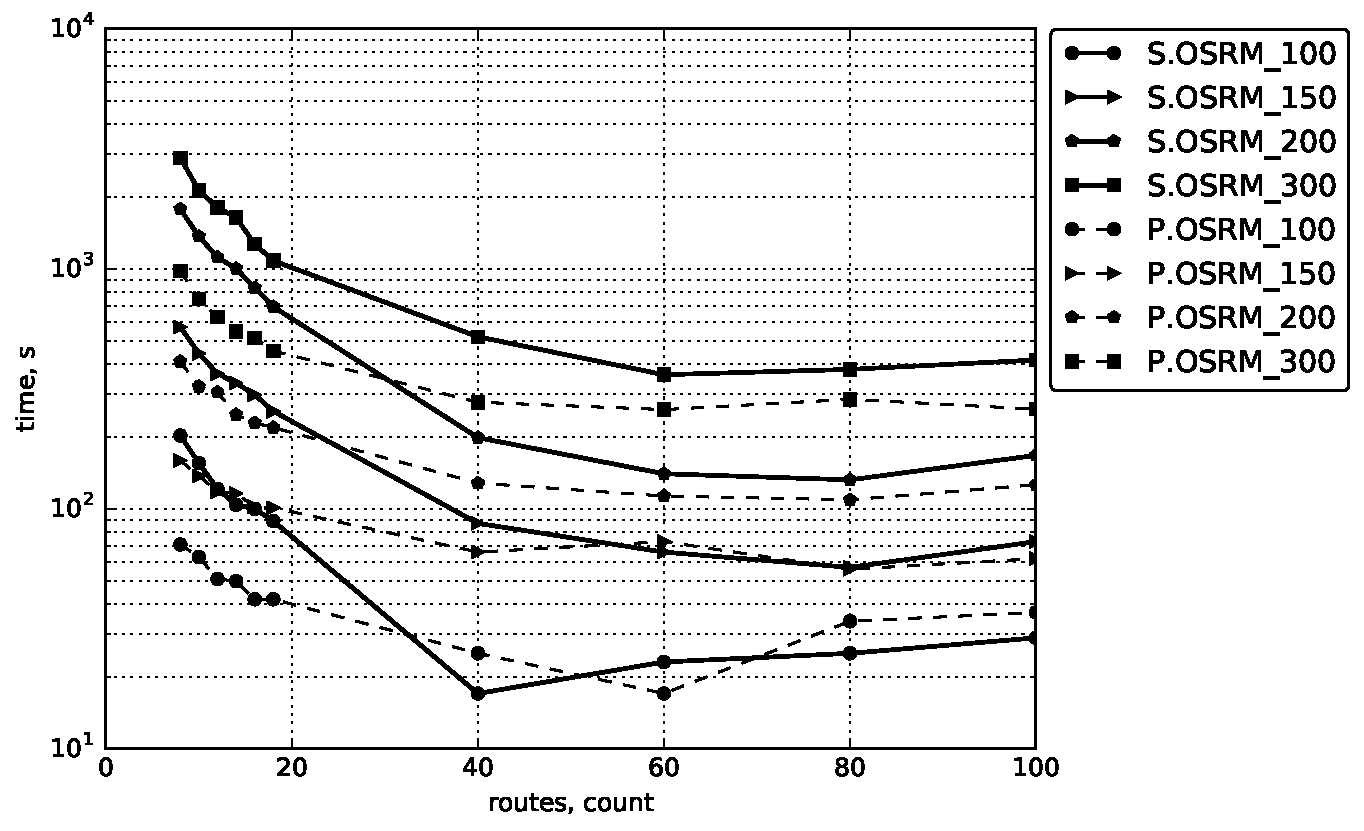
\includegraphics[width=\textwidth]{result-01}
    \caption{Зависимость времени построения от количества маршрутов}
    \label{fig:result-01}
\end{figure}

\begin{figure}[t!]
    \centering
    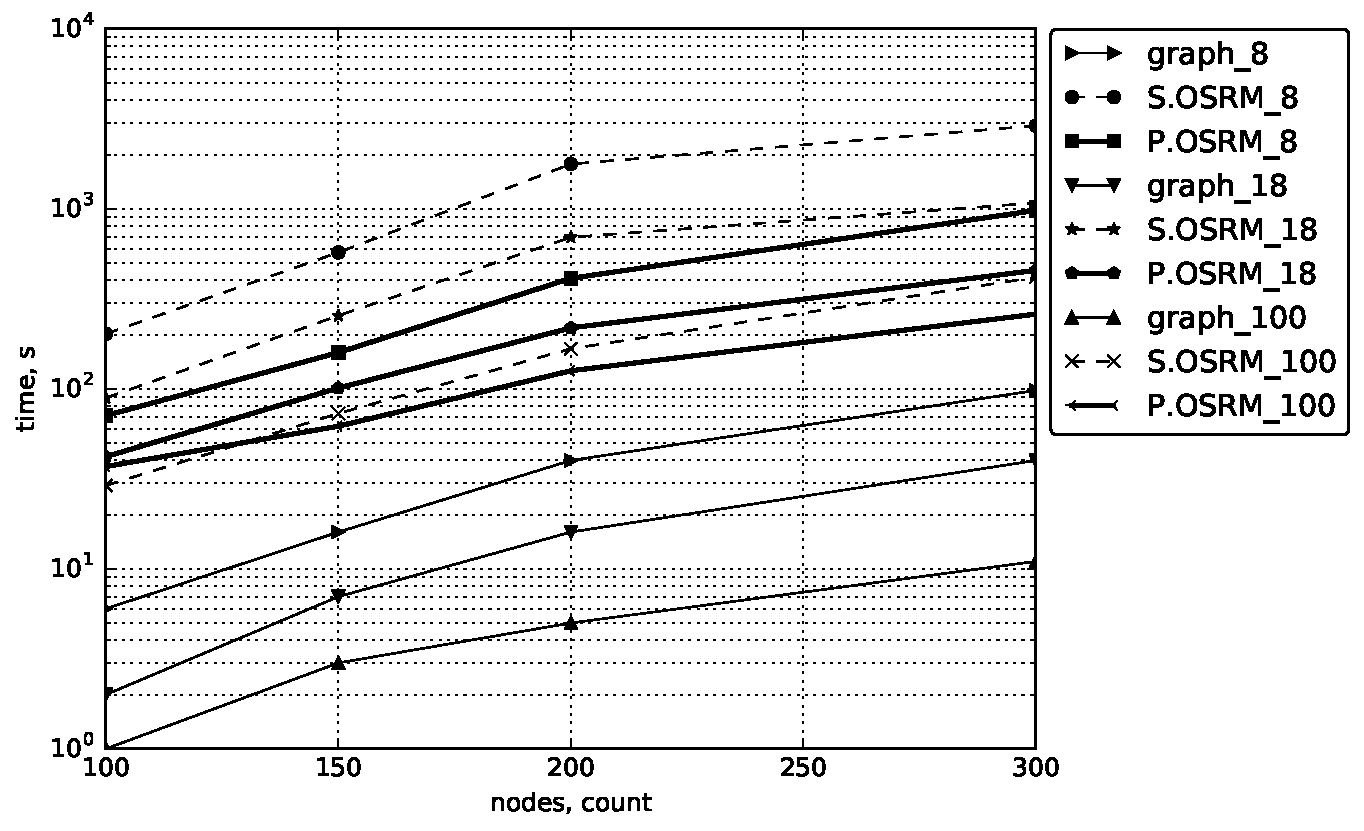
\includegraphics[width=\textwidth]{result-02}
    \caption{Зависимость времени построения от кластеров}
    \label{fig:result-02}
\end{figure}

\begin{table*}[h!]
    \centering
    \caption{Результаты эксперимента алгоритма из пункта \ref{sec:second_alg}}
    \label{tab:second_alg}
    \small
    \begin{tabular}{|c|l|c|c|c|c|c|c|l|l|l|c|}
        \hline
        \multicolumn{1}{|l|}{}      &          & \multicolumn{10}{c|}{routes}                                                                                                       \\ \hline
        \multicolumn{1}{|l|}{nodes} & strategy & 8     & 10    & 12    & 14    & 16    & 18    & \multicolumn{1}{c|}{40} & \multicolumn{1}{c|}{60} & \multicolumn{1}{c|}{80} & 100  \\ \hline
        \multirow{3}{*}{100}        & graph    & 0:06  & 0:04  & 0:03  & 0:03  & 0:02  & 0:02  & 0:01                    & 0:01                    & 0:01                    & 0:01 \\ \cline{2-12} 
        & S. OSRM  & 3:22  & 2:35  & 2:01  & 1:44  & 1:40  & 1:29  & 0:17                    & 0:23                    & 0:25                    & 0:29 \\ \cline{2-12} 
        & P. OSRM  & 1:11  & 1:03  & 0:51  & 0:50  & 0:42  & 0:42  & 0:25                    & 0:17                    & 0:34                    & 0:37 \\ \hline
        \multirow{3}{*}{150}        & graph    & 0:16  & 0:12  & 0:10  & 0:08  & 0:07  & 0:07  & 0:04                    & 0:03                    & 0:02                    & 0:03 \\ \cline{2-12} 
        & S. OSRM  & 9:32  & 7:24  & 6:06  & 5:34  & 4:59  & 4:15  & 1:27                    & 1:06                    & 0:57                    & 1:13 \\ \cline{2-12} 
        & P. OSRM  & 2:39  & 2:17  & 1:58  & 1:56  & 1:42  & 1:41  & 1:06                    & 1:13                    & 0:56                    & 1:02 \\ \hline
        \multirow{3}{*}{200}        & graph    & 0:40  & 0:31  & 0:25  & 0:20  & 0:20  & 0:16  & 0:08                    & 0:06                    & 0:05                    & 0:05 \\ \cline{2-12} 
        & S. OSRM  & 29:33 & 22:45 & 18:36 & 16:43 & 13:53 & 11:35 & 3:18                    & 2:20                    & 2:12                    & 2:47 \\ \cline{2-12} 
        & P. OSRM  & 6:51  & 5:23  & 5:06  & 4:07  & 3:48  & 3:38  & 2:08                    & 1:53                    & 1:49                    & 2:06 \\ \hline
        \multirow{3}{*}{300}        & graph    & 1:38  & 1:16  & 1:02  & 0:51  & 0:46  & 0:40  & 0:20                    & 0:14                    & 0:11                    & 0:11 \\ \cline{2-12} 
        & S. OSRM  & 48:20 & 35:24 & 30:00 & 27:17 & 21:06 & 18:01 & 8:41                    & 6:02                    & 6:21                    & 6:57 \\ \cline{2-12} 
        & P. OSRM  & 16:20 & 12:28 & 10:31 & 9:08  & 8:35  & 7:35  & 4:38                    & 4:19                    & 4:46                    & 4:20 \\ \hline
    \end{tabular}
\end{table*}
% Данные в таблице представлены в формате минуты:секунды

\section{Обсуждение результатов}
\section{Интеграция}

\section{Заключение}